\begin{frame}{Main steps of MCTS}
    \begin{center}
        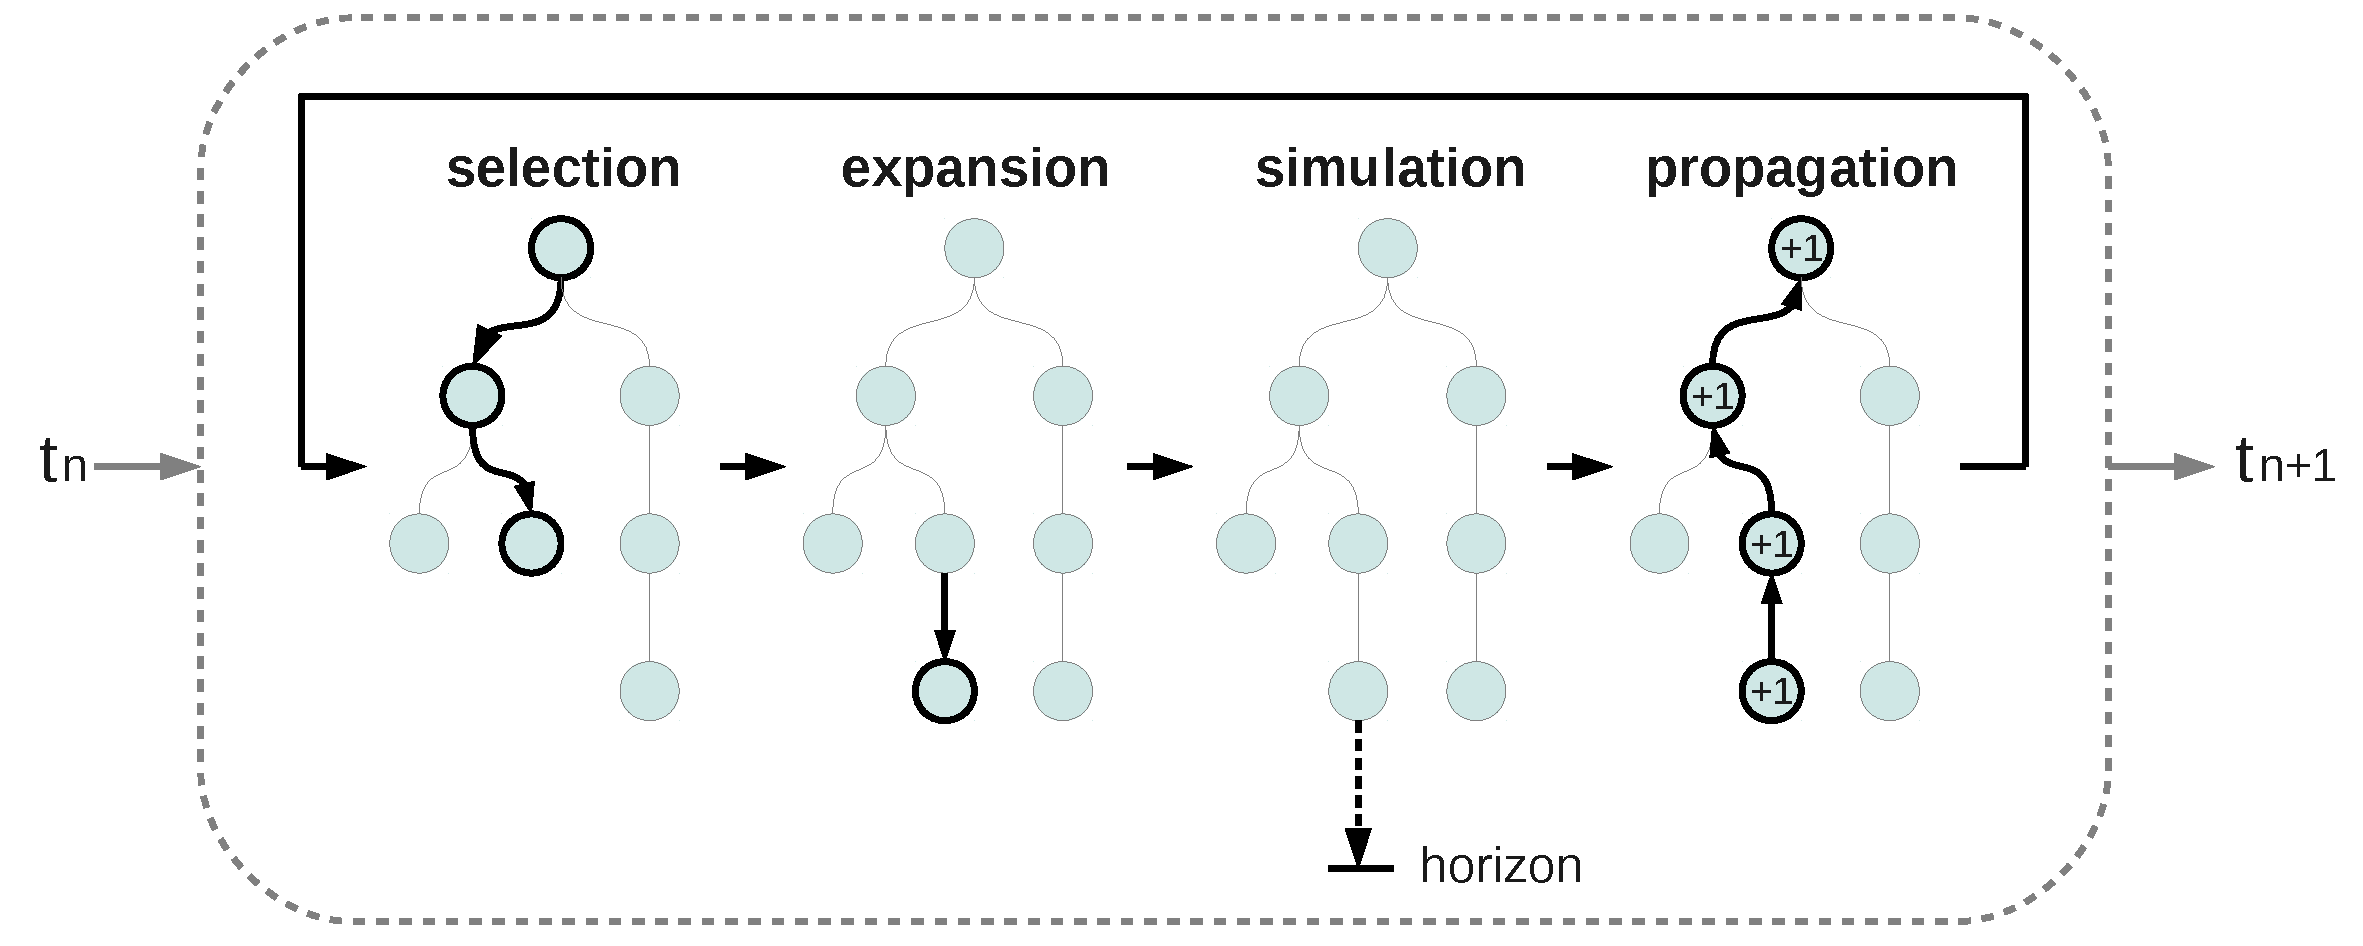
\includegraphics[width=.99\linewidth]{figs/tree9}
    \end{center}
\end{frame}


\begin{frame}{Main steps of MCTS}
    \only<1| handout:0> {
        \begin{center}
            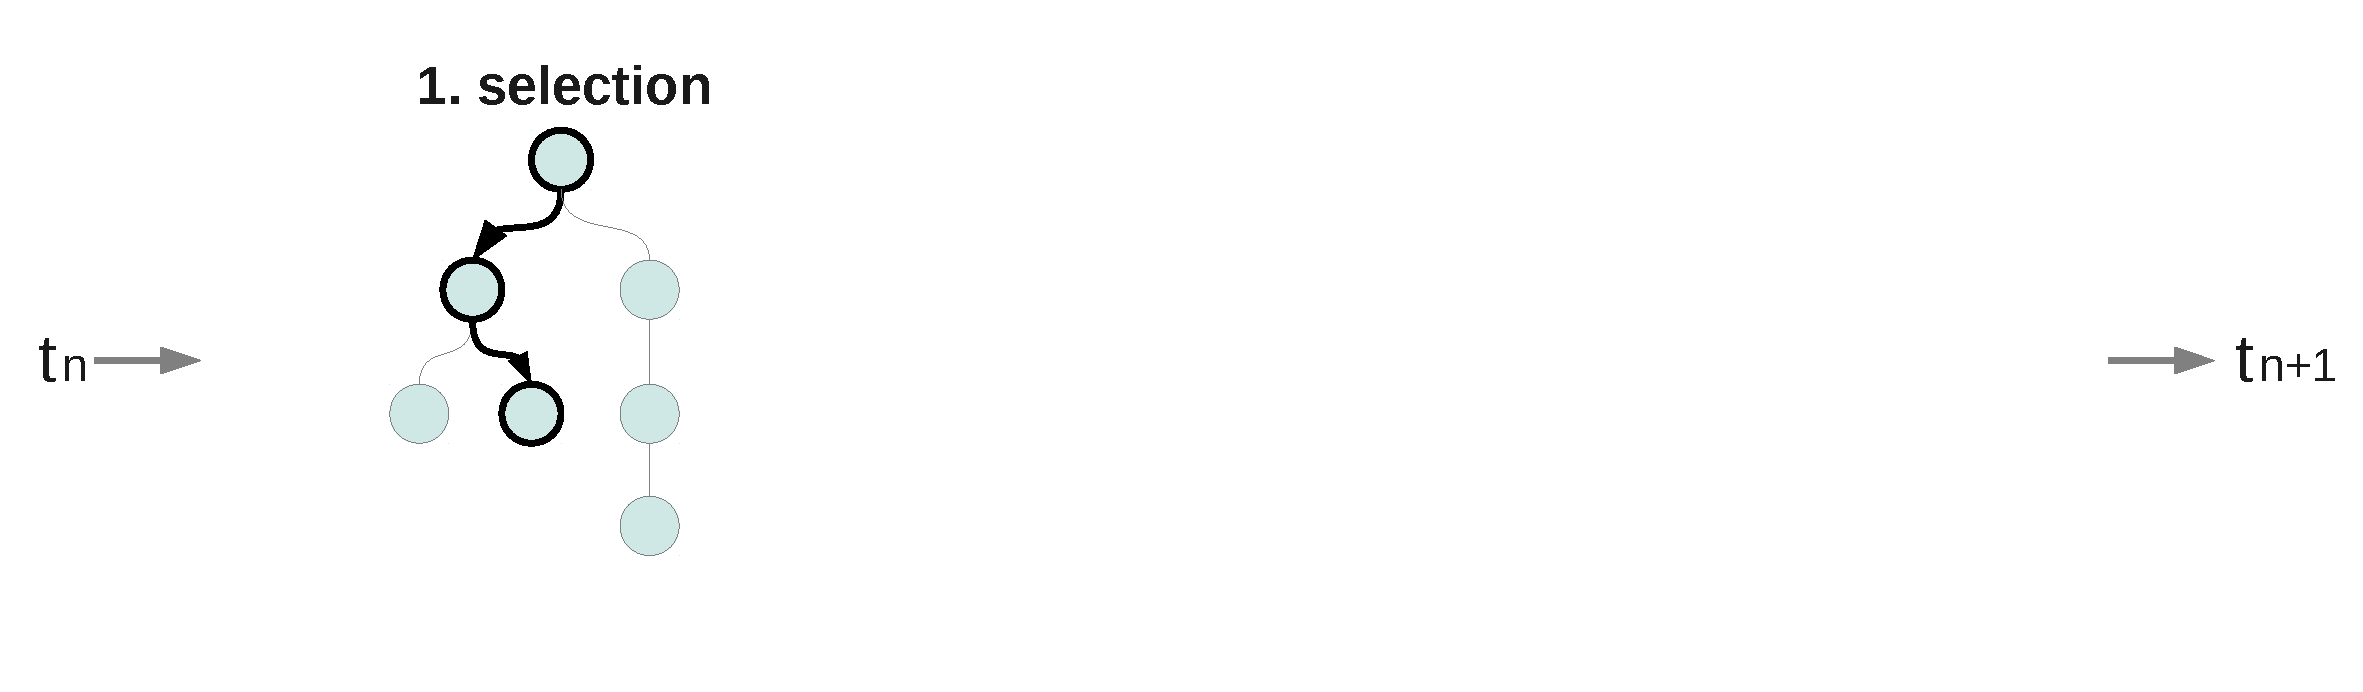
\includegraphics[width=.75\linewidth]{figs/tree10a}
        \end{center}
    }
    \only<2| handout:0> {
        \begin{center}
            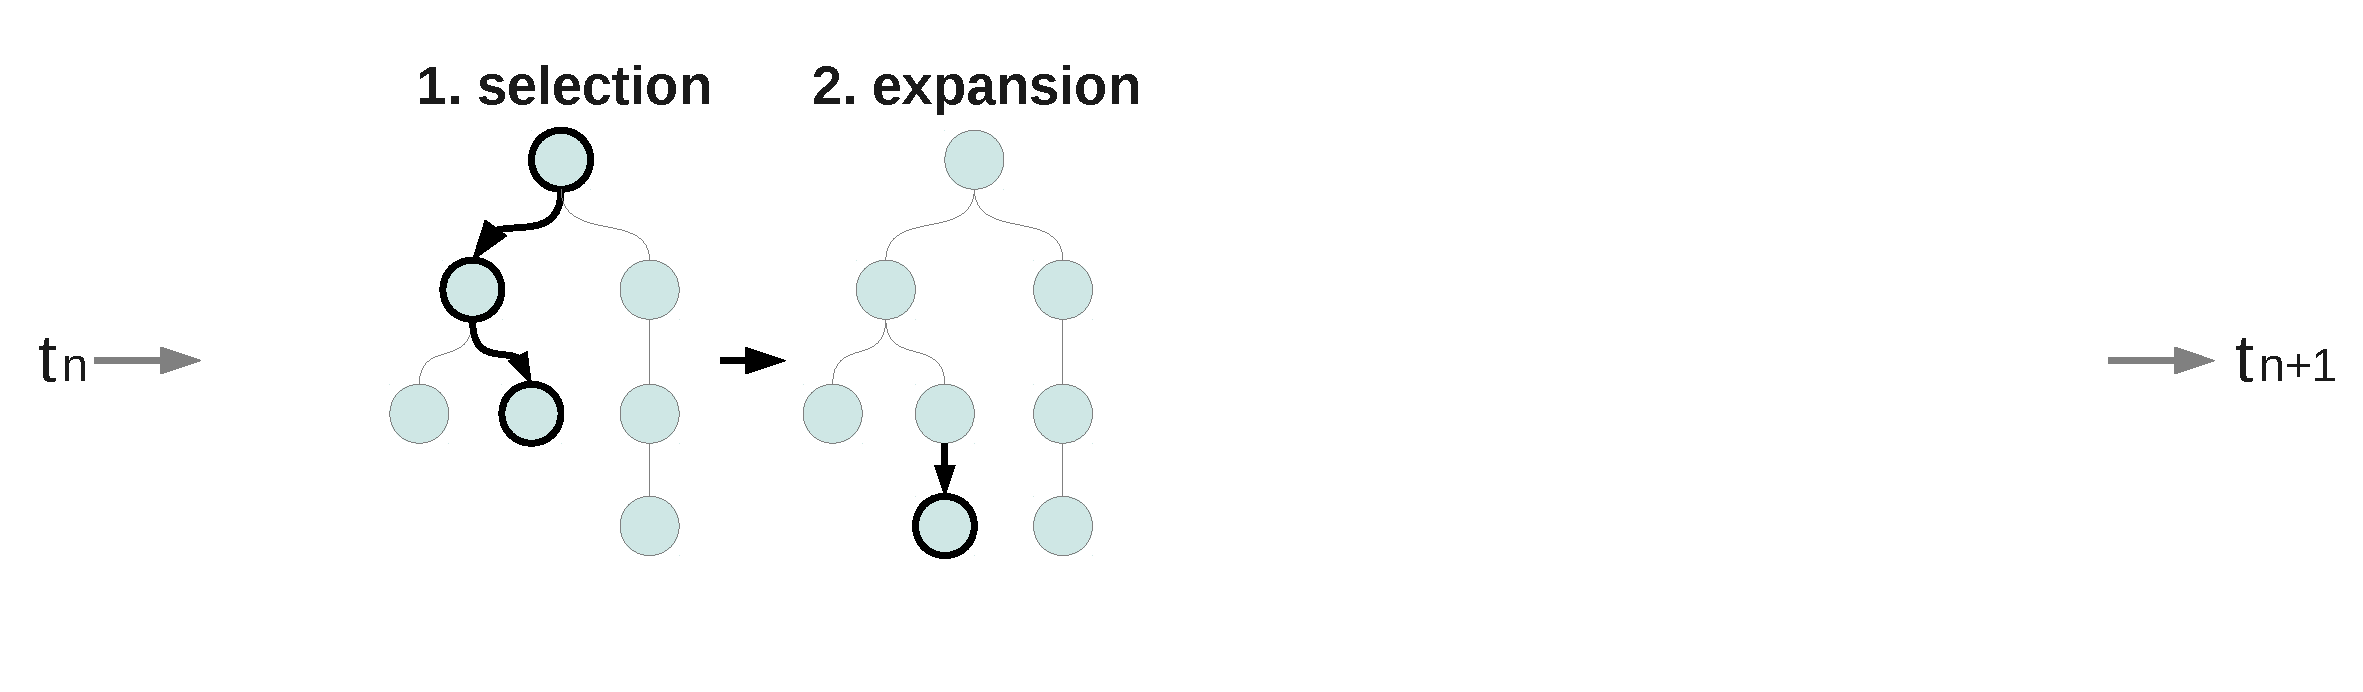
\includegraphics[width=.75\linewidth]{figs/tree10b}
        \end{center}
    }
    \only<3| handout:0> {
        \begin{center}
            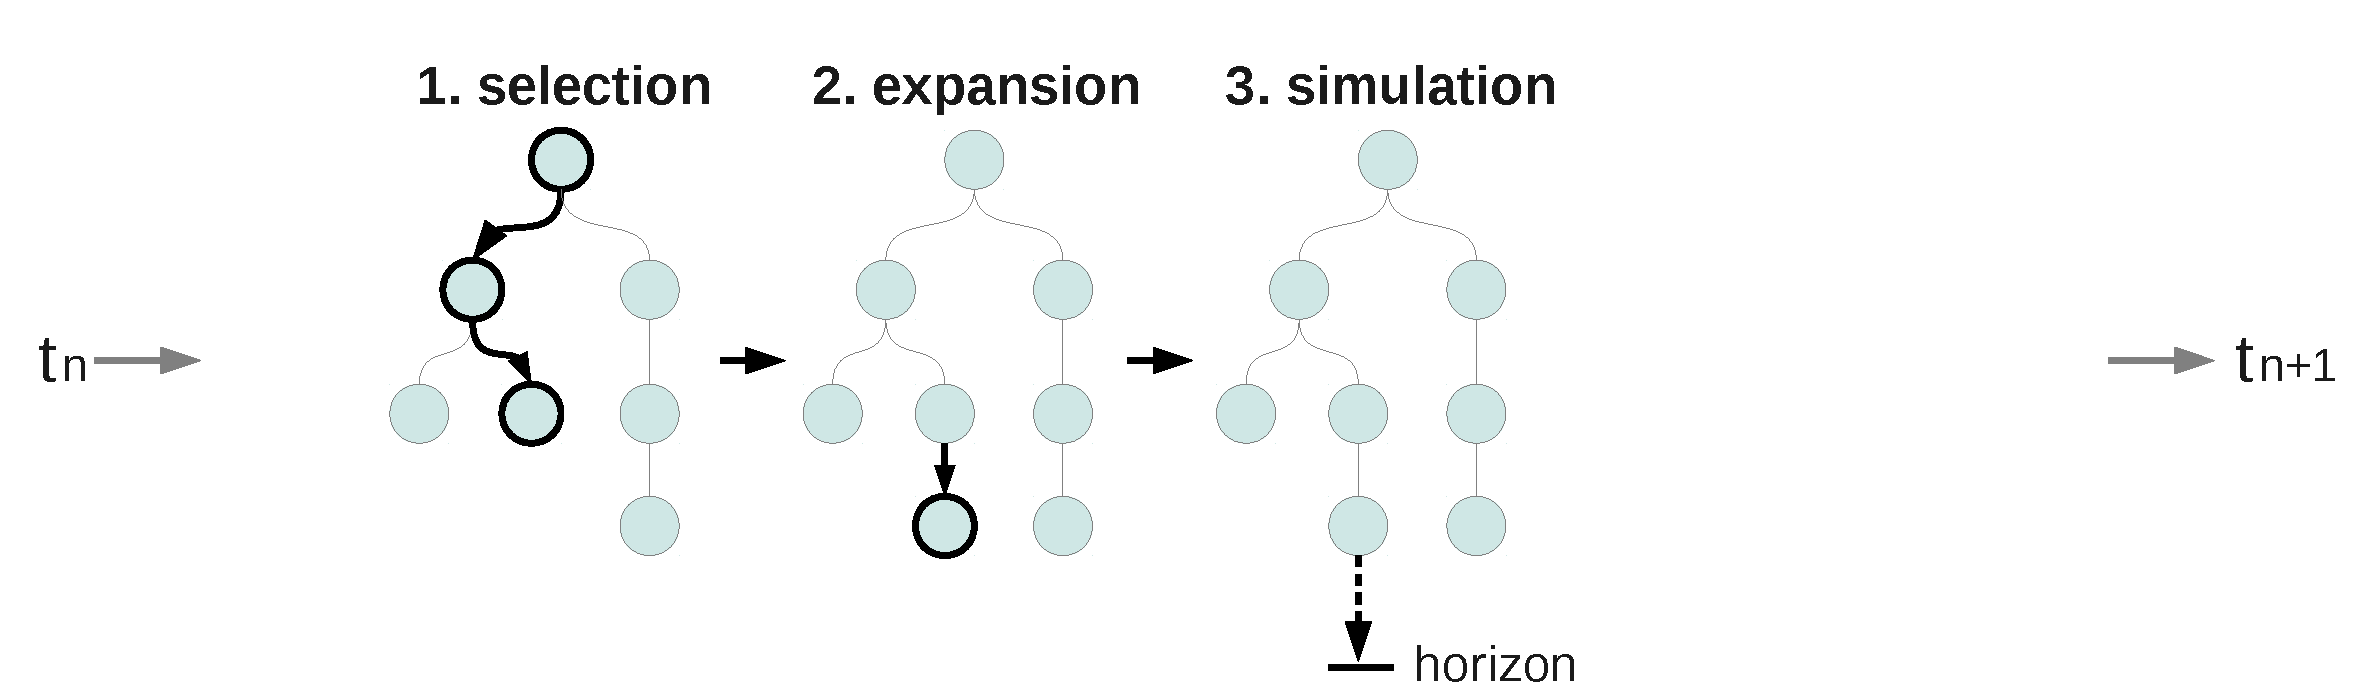
\includegraphics[width=.75\linewidth]{figs/tree10c}
        \end{center}
    }
    \only<4| handout:0> {
        \begin{center}
            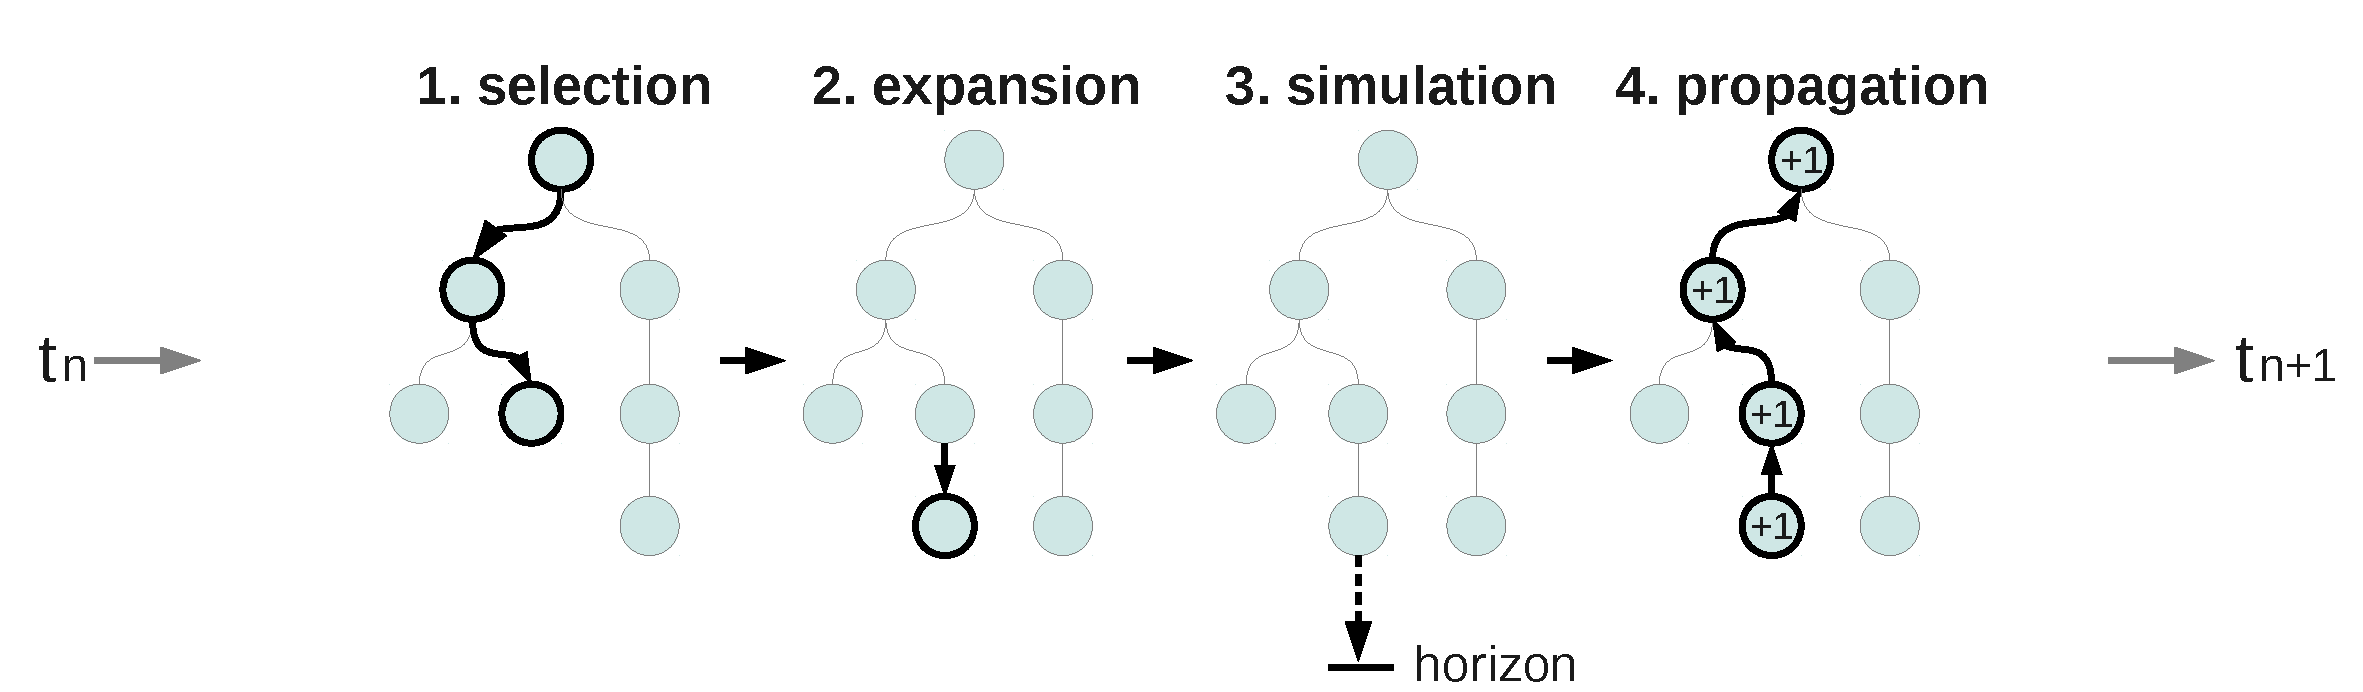
\includegraphics[width=.75\linewidth]{figs/tree10d}
        \end{center}
    }
    \only<5> {
        \begin{center}
            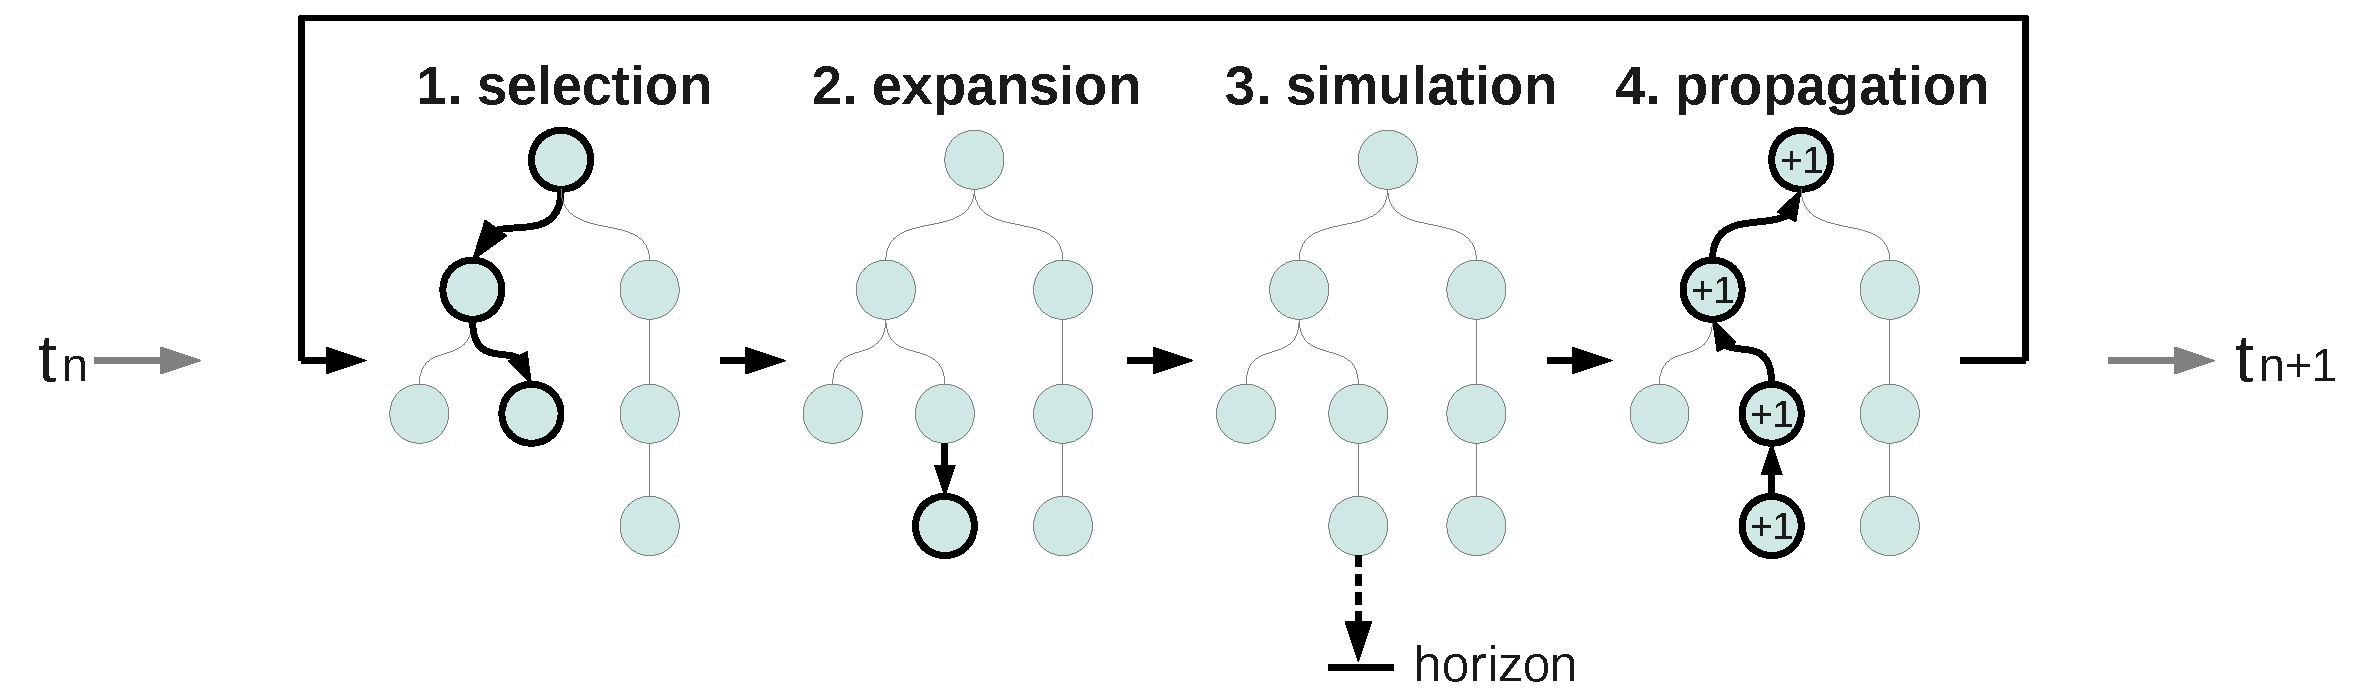
\includegraphics[width=.75\linewidth]{figs/tree10e}
        \end{center}
    }
    \begin{small}
        Starting from an initial state:%, repeat next steps until time budget is over:
        \begin{enumerate}
            \item<1-> select the state we want to expand from
            \item<2-> add the generated state in memory
            \item<3-> evaluate the new state with a default policy until horizon is reached
            \item<4-> back-propagation of some information:
            \begin{itemize}
                \item $n(\state,\decision)$ : number of times decision $\decision{}$ has been simulated in $\state$
                \item $n(\state)$ : number of time $\state$ has been visited in simulations
                \item $\hat{Q}(\state,\decision)$ : mean reward of simulations where $\decision$ was whosen in $\state$
            \end{itemize}
        \end{enumerate}
        ~\\
    \end{small}
\end{frame}


\begin{frame}{Main steps of MCTS}
    \begin{center}
        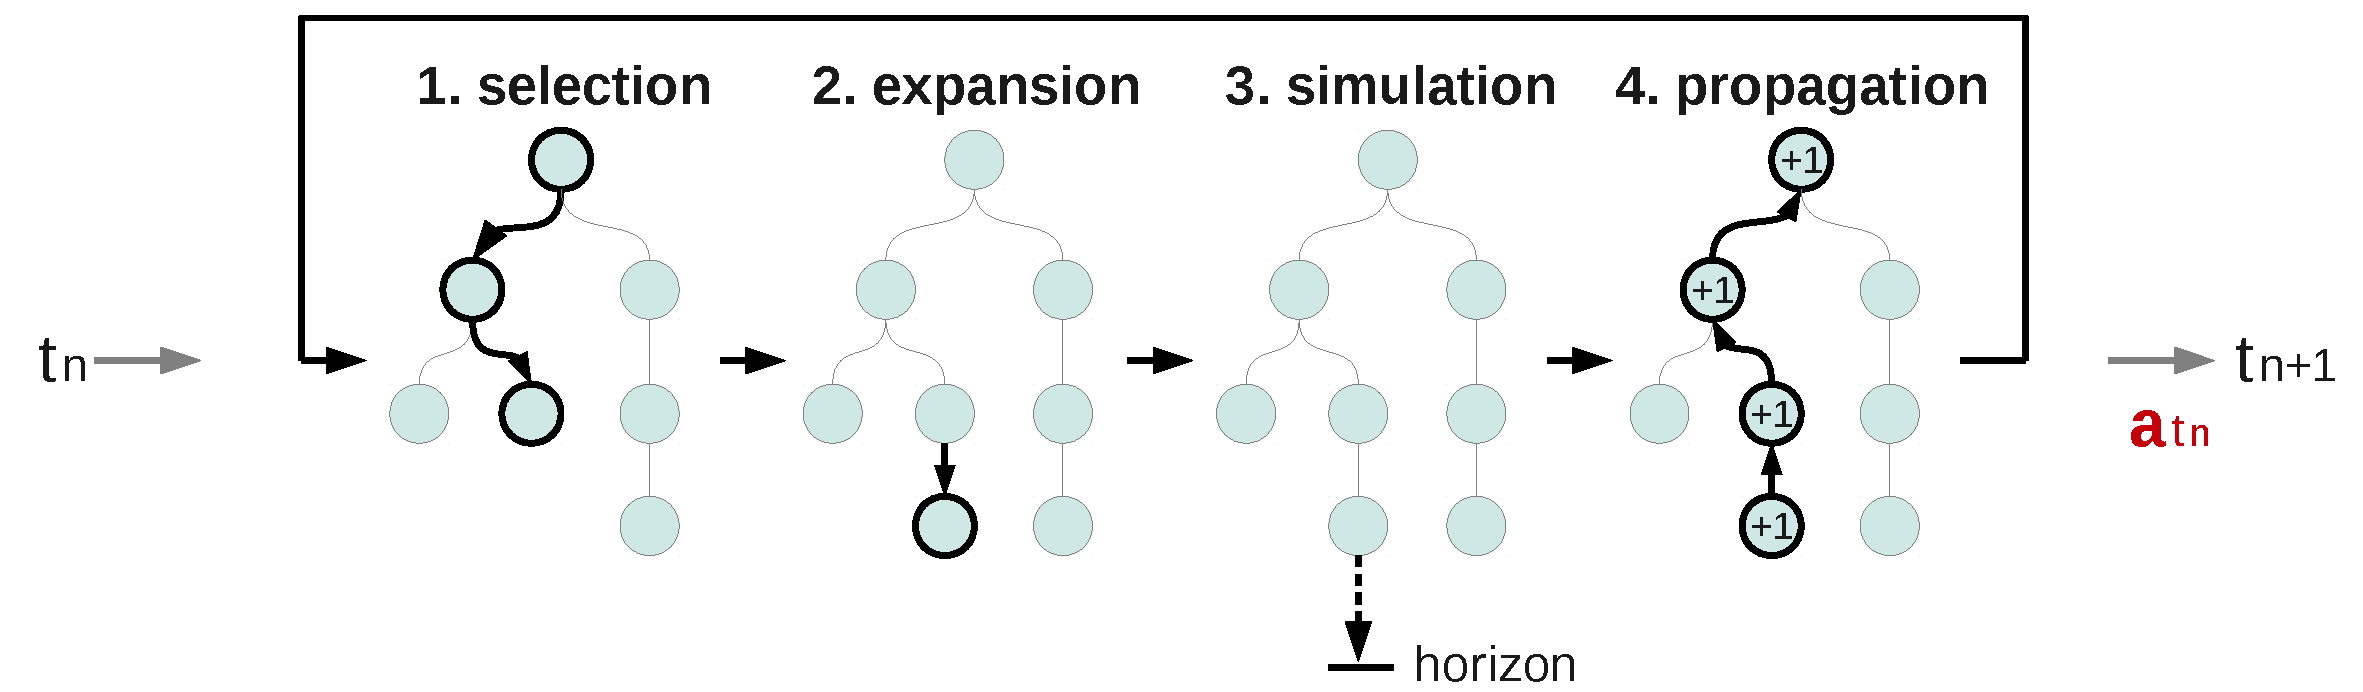
\includegraphics[width=.75\linewidth]{figs/tree10f}
    \end{center}

    \begin{block}{The selected decision}
        $\decision_{t_n}$ = the most visited decision form the current state (root node)
    \end{block}
\end{frame}
